\documentclass[11pt,letterpaper]{article}
\usepackage[lmargin=1in,rmargin=1in,tmargin=0.75in,bmargin=1in]{geometry}

% -------------------
% Packages
% -------------------
\usepackage{
	amsmath,			% Math Environments
	amssymb,			% Extended Symbols
	enumerate,		% Enumerate Environments
	graphicx,			% Include Images    
	lastpage,			% Reference Lastpage
	multicol,			% Use Multi-columns
	multirow,			% Use Multi-rows
	siunitx
}

\graphicspath{{./images/}}

\usepackage{wrapfig}

% -------------------
% Font
% -------------------
\usepackage[T1]{fontenc}
\usepackage{charter}    


% -------------------
% Heading Commands
% -------------------
\thispagestyle{empty}
\vspace*{-0.5in}

\begin{minipage}{\textwidth}
     \begin{center}
          \textbf{\huge AMC 8 Cheat Sheet}
          \vspace{0.1in}
     \end{center}
\end{minipage} \\
\rule[2ex]{\textwidth}{2pt} 

% -------------------
% Commands
% -------------------

\newcommand{\pspace}{\par\vspace{\baselineskip}}
\newcommand{\ds}{\displaystyle}

% -------------------
% Content
% -------------------

\begin{document}
\centering
\begin{minipage}{\textwidth}
     \noindent \textbf{Test Taking Strategies}
     \begin{itemize}
          \item Try Solving the problem first
          \item Substitute answer choices
          \item Try to find patterns with smaller numbers
          \item Use your tools
           \begin{itemize}
               \item You can use rulers, compasses, and protractors to draw and estimate lengths and angle measure. Be aware that picture problems are not drawn exactly to scale
               \item Use graph paper to graph equations to estimate possible solutions
          \end{itemize}
          \item Eliminate some options 
          \begin{itemize}
               \item narrow down to 1 choice to find the solution
               \item increase probability of guesses
          \end{itemize}
          \item Last resort is to guess
          \item NEVER LEAVE A QUESTION BLANK, you won't be penalized; you can only benefit
          
     \end{itemize}

\end{minipage}


\vspace{0.4cm}

\begin{minipage}{\textwidth}
     \noindent \textbf{Geometry}
     \begin{center}
          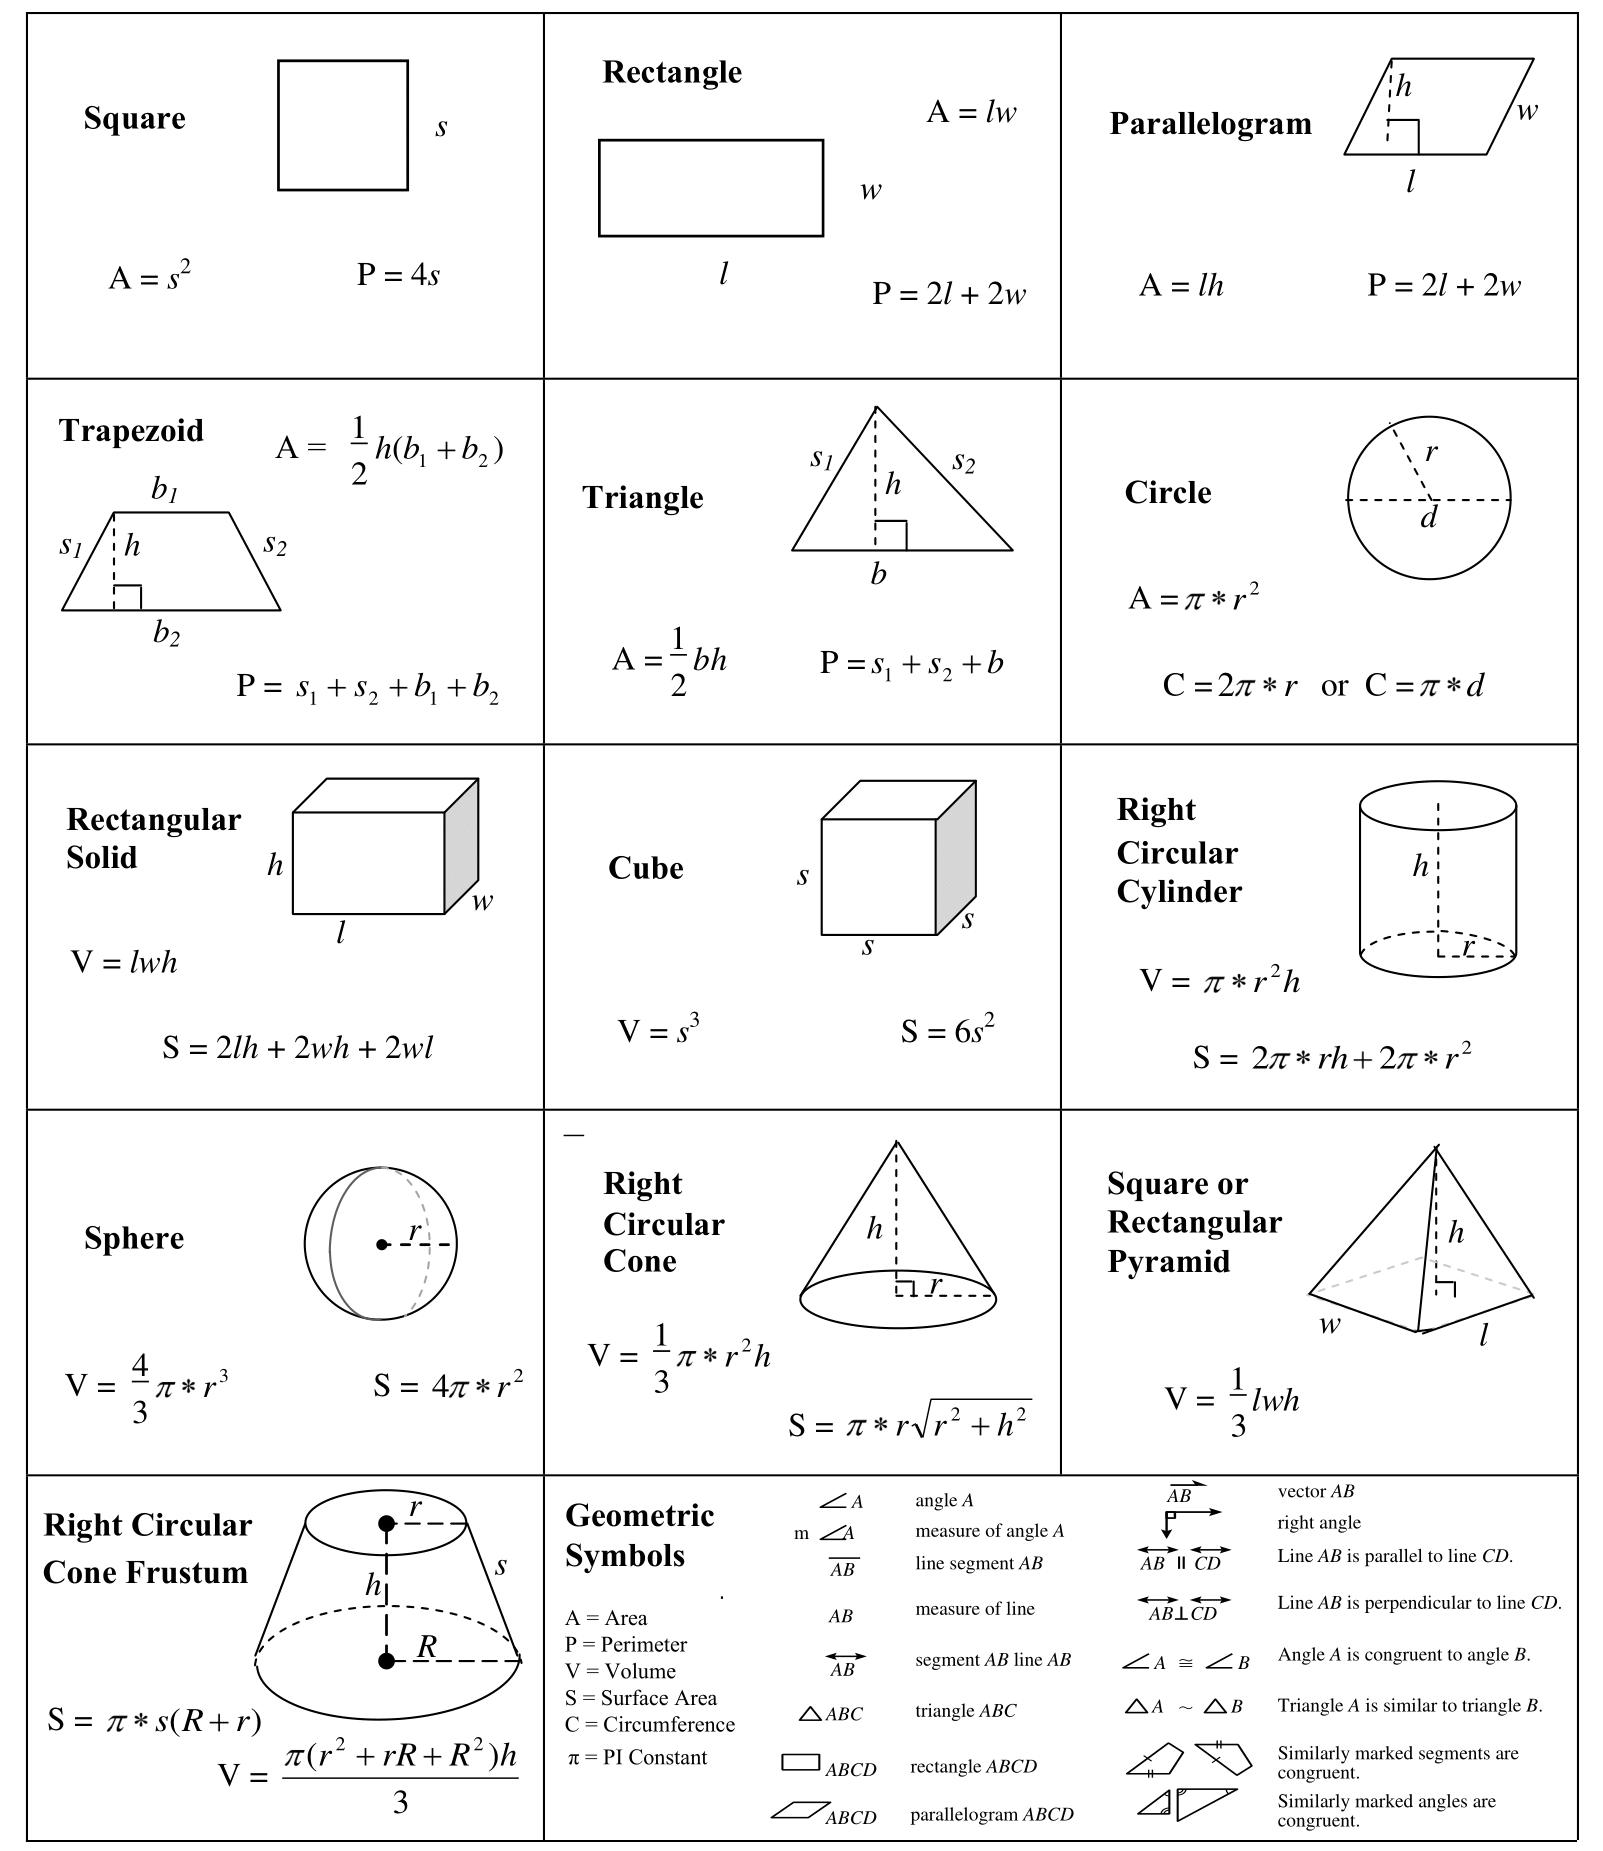
\includegraphics[height = 13cm]{images/geometry.png}
     \end{center}    
\end{minipage}

\vspace{15cm}

\begin{minipage}{\textwidth}
     \begin{itemize}
          \item Angle pair relationships
          \begin{itemize}
               \item Adjacent - angles that neighbor each other; bisected by a single line
               \item Complementary - Angles that add up to $90^{\circ}$
               \item Supplementary / linear pair -  Angles that add up to $180^{\circ}$; along a straight line
               \item Vertical - pairs of opposite angles made by two intersecting lines
               
               \vspace{0.2cm}
               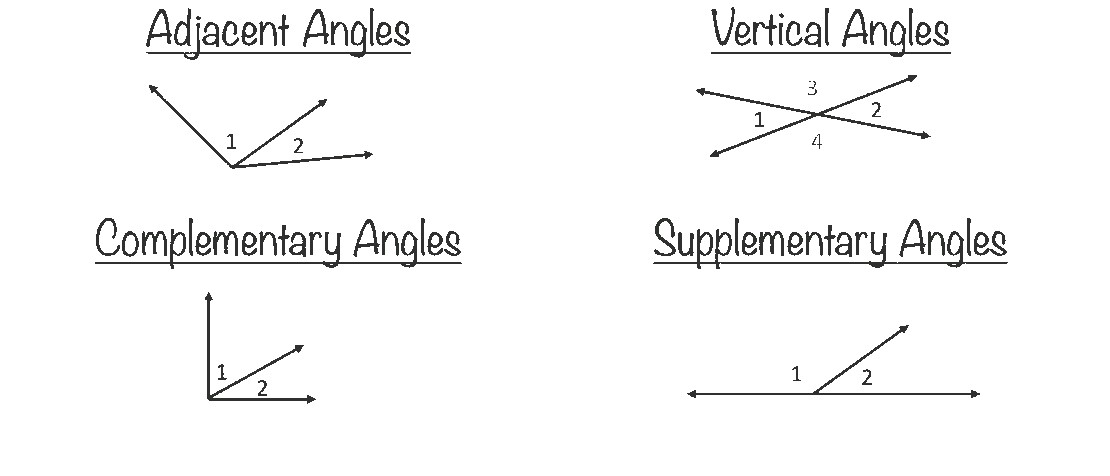
\includegraphics[height = 7cm]{images/anglrel.jpg}
          \end{itemize}
          \vspace{-0.5cm}
          \item Triangles
          \begin{itemize}
               \item When a triangle has an angle of $90^{\circ}$ the sum of the squared legs of a triangle is equal to the squared hypotenuse; $a^2+b^2=c^2$
               \item The numbers that are possible for the values of $a$, $b$, &$c$ are known as pythagorean triples. Common triples include:
               \begin{itemize}
                    \item $3$, $4$, $5$
                    \item $5$, $12$, $13$
                    \item $6$, $8$, $10$
                    \item $7$, $24$, $25$
                    \item $9$, $12$, $15$
                    
               \end{itemize}
          \end{itemize}
          \item Circles
          \begin{itemize}
               \item The area of a sector = $\frac{\pi r^2\theta}{360^{\circ}}$
               \item The length of an arc = $\frac{2\pi r\theta}{360^{\circ}}$
          \end{itemize}
          \item Polygons
          \begin{itemize}
               \item The sum of the interior angles of any polygon = $(number of sides-2) * 180$
               \item The measure of an interior angle of a regular polygon = $\frac{n-2}{n} * 180$
               \item The measure of an exterior angle of a regular polygon = $\frac{360}{n}$
          \end{itemize}
        \end{itemize} 
\end{minipage}

\vspace{0.4cm}

\begin{minipage}{\textwidth}
     \noindent \textbf{Common Situations / Vocabulary}
     \begin{itemize}
          \item Mean - the average value for a data set = $\frac{Sum of all Terms}{Number of Terms}$
          \item Median - the point lying in the middle of a data set; exactly 1/2 on either side
          \item Mode - the most common number in a data set
          \item Speed - $\frac{Distance}{Time}$
          \item Distance - $Speed * Time$
          \item Combinations - Formula for choosing $k$ objects from $n$ =${{n}\choose {k}} = \frac {n!} {k!(n-k)!}$
          \item Number of integer multiples of $a,b,c$ that are less than or equal to $x$ = $\frac{a}{x} + \frac{c}{x} + \frac{b}{x} -\frac{ab}{x} + \frac{ac}{x} + \frac{bc}{x} $
     \end{itemize}
\end{minipage}

\begin{minipage}{\textwidth}
     \vspace{0.4cm}
     \noindent \textbf{Systems of equations}\\
     A system of equations is a set of equations which share the same variables. Below is an example of a system of equations.
     \begin{itemize}
          \item Elimination
          \begin{itemize}
               \item  Elimination involves eliminating variables from the system by adding constant multiples of two or more of the equations together. Let's look at an example:

               Problem
               Find the ordered pair $(x,y)$ for which
               
               \[\left\{\begin{array}{l}x-12y=2\\3x+6y=6\end{array}\right.\]
               Solution
               We can eliminate $y$ by adding twice the second equation to the first:
               
               $x - 12y= 2$
               $+2($	$3x + 6y = 6)$
               simplifying we get ${7x + 0=14}$
               Thus $x=2$. We can then plug in for $x$ in either of the equations:\begin{align*} (2)-12y &= 2 \\ y &= 0 \end{align*}
               Thus, the solution to the system is $(2,0)$.
          \end{itemize}
          \item Substitution
          \begin{itemize}
               \item Substitution requires solving for a variable and then plugging that variable into another equation therefore reducing the number of variables. We'll show how to solve the same problem from the elimination section using substitution.

               Problem
               Find the ordered pair $(x,y)$ for which
               
               \[\left\{\begin{array}{l}x-12y=2\\3x+6y=6\end{array}\right.\]
               Solution
               The first equation can be solved for $x$:
               
               $x = 12y + 2.$
               Plugging this into the second equation yields
               
               $3(12y + 2) + 6y = 6 \Leftrightarrow 42 y = 0.$
               Thus $y=0$. Plugging this into either of the equations and solving for $x$ yields $x=2$.
          \end{itemize}
     \end{itemize}
\end{minipage}
\vspace{0.4cm}
\begin{minipage}{\textwidth}
     \noindent \textbf{Sum of geometric sequences}
     \begin{itemize}
          \item In algebra, a geometric sequence, sometimes called a geometric progression, is a sequence of numbers such that the ratio between any two consecutive terms is constant. This constant is called the common ratio of the sequence.

          For example, $1, 2, 4, 8$ is a geometric sequence with common ratio $2$ and $100, -50, 25, -25/2$ is a geometric sequence with common ratio $-1/2$; however, $1, 3, 9, -27$ and $-3, 1, 5, 9, \ldots$ are not geometric sequences, as the ratio between consecutive terms varies.
          
          More formally, the sequence $a_1, a_2, \ldots , a_n$ is a geometric progression if and only if $a_2 / a_1 = a_3 / a_2 = \cdots = a_n / a_{n-1}$. A similar definition holds for infinite geometric sequences. It appears most frequently in its three-term form: namely, that constants $a$, $b$, and $c$ are in geometric progression if and only if $b / a = c / b$.
          \item Finite
          \begin{itemize}
               \item A finite geometric series with first term $a_1$, common ratio $r$ not equal to one, and $n$ total terms has a value equal to $\frac{a_1(r^n-1)}{r-1}$.
          \end{itemize}
          \item Infinite 
          \begin{itemize}
               \item An infinite geometric series converges if and only if $|r|<1$; if this condition is satisfied, the series converges to $\frac{a_1}{1-r}$.
          \end{itemize}
     \end{itemize}
\end{minipage}
\begin{minipage}{\textwidth}
     \noindent \textbf{Guessing Strategies}
     \begin{itemize}
          \item If you can’t solve, here are some tips on guessing
          \item Sometimes you can eliminate
          \begin{itemize}
               \item answer choices too large or too small
               \item answer choices odd or even
               \item answer choices divisible by $x$
          \end{itemize}
          \item In geometry problems, estimate the dimensions
          \begin{itemize}
               \item figures are not to scale, but they are close
               \item Graph paper, rulers, and protractors are allowed
          \end{itemize}
          \item Make sure to mark an answer for every problem($20\%$ chance of getting it right)
        \end{itemize}
\end{minipage}





\end{document}
